% From mitthesis package
% Version: 1.07, 2024/09/26
% Documentation: https://ctan.org/pkg/mitthesis

\lstdefinestyle{mystyle}{
    backgroundcolor=\color{CadetBlue!15!white},   
    commentstyle=\color{Red3},
    numberstyle=\tiny\color{gray},
    stringstyle=\color{Blue3},
    basicstyle=\small\ttfamily,
    breakatwhitespace=false,         
    breaklines=true,                 
    numbers=left,                    
    numbersep=5pt,                  
    showspaces=false,                
    showstringspaces=false,
    showtabs=false,                  
    tabsize=2,
    language=C
}%
\lstset{language=C,style={mystyle}}%

\chapter{Problemas comunes}

\section{Acceso al hardware}
\label{Accesoalhardware}
Una de las características distintivas de los sistemas embebidos es que trabajan directamente con dispositivos de hardware. Cada uno de estos tiene sus propios protocolos de comunicación y estándares de funcionamiento (por ejemplo, direcciones de memoria, codificación de bits, etc), por lo tanto el software se debe ajustar a sus requerimientos. Como se puede entender esta tarea no es simple y puede demandar mucho esfuerzo cada vez que se quiera modificar o agregar un componente de hardware. A su vez, puede que múltiples módulos de nuestro sistema embebido quieran acceder al dispositivo, por lo que cada uno debe encargarse de la comunicación creando código repetido y complicando aún más las modificaciones. 

Para entender los inconvenientes que puede conllevar no diseñar pensando en el cambio veamos un ejemplo simple. Suponga que nuestro sistema embebido debe controlar un motor de corriente continua (DC) y que el software para hacerlo corre en un microcontrolador Arduino. Los requerimientos definen que es necesario poder asignar el sentido y la velocidad de rotación del motor según se necesite. Para controlar el motor se utiliza un módulo \textit{DRV8838}, el cual se coloca entre el microcontrolador y el motor. Es necesario ya que el microcontrolador y su plataforma no pueden manejar las potencias necesarias para hacer funcionar el dispositivo. Podemos ver el conexionado del mismo en la figura \ref{drv8838}.

\begin{figure}[h]
    \centering
    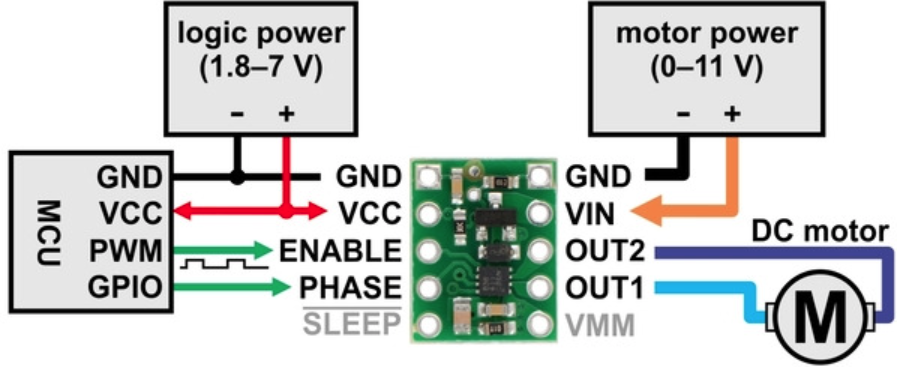
\includegraphics[width=0.65\linewidth]{drv8838.png}
    \caption{Conexionado módulo DRV8838}
    \label{drv8838}
\end{figure}

Notemos que el DRV8838 tiene 3 pines de control, \textit{ENABLE}. \textit{PHASE} y \textit{SLEEP} pero solo utilizaremos los 2 primeros para simplificar el ejemplo. De todas formas, en esta tabla \ref{funciones_pin_drv8838} podemos ver la función de cada pin.


\begin{table}[h]
\centering
\begin{tabular}{lllll}
\cline{1-3}
\multicolumn{1}{|l|}{PHASE}  & \multicolumn{1}{l|}{direccion de rotacion} & \multicolumn{1}{l|}{digital}   &  &  \\ \cline{1-3}
\multicolumn{1}{|l|}{ENABLE} & \multicolumn{1}{l|}{velocidad de rotación} & \multicolumn{1}{l|}{analogico} &  &  \\ \cline{1-3}
\multicolumn{1}{|l|}{SLEEP}  & \multicolumn{1}{l|}{liberar fuerza}        & \multicolumn{1}{l|}{digital}   &  &  \\ \cline{1-3}
                             &                                            &                                &  & 
\end{tabular}
\caption{Funciones de cada pin del módulo DRV8838}
\label{funciones_pin_drv8838}
\end{table}

Por lo tanto, con los dos primeros pines podremos cumplir los requerimientos mencionados. \textbf{•}, tendremos dos cables conectados a nuestro microcontrolador \textbf{Arduino}, uno que se dirige a \textit{ENABLE} y otro a \textit{PHASE}. Veamos ahora que código \ref{listing1} necesitamos escribir para poder hacer uso del motor.

\begin{lstlisting}[caption=Configuración inicial,label={listing1}]
# Notar que los numeros asignados a los pines son arbritarios dentro del conjunto de pines disponibles en nuestro Aruino.

# Constantes globales
const int DIR\_pin = 7;
const int VEL\_pin = 9;

void setup() {
     .
     .
     .
  pinMode(DIR\_pin, OUTPUT);
  pinMode(VEL\_pin, OUTPUT);
     .
     .
     .
}
\end{lstlisting}

\begin{lstlisting}[caption=Máxima velocidad giro horario]
digitalWrite(DIR\_pin, HIGH);
analogWrite(VEL\_pin, 255); # Maximo valor aceptado, PWM siempre encendido
\end{lstlisting}

\begin{lstlisting}[caption=Detenerce]
analogWrite(VEL\_pin, 0);
\end{lstlisting}

No es necesario entender por completo que hace cada llamada, pero si es importante comprender que es necesario ejecutar ese código para controlar el motor. Es decir, que si cualquier cliente (se supone que ya definimos que es cliente) del motor en nuestro sistema deberá saber que para hacer que el motor vaya hacia adelante a la mayor velocidad posible es necesario ejecutar las dos funciones indicadas sobre los pines correspondientes al motor. Un pequeño ejemplo podría ser el siguiente \ref{listingMotor}, en el cual se consulta una bandera asociada al estado de un valor y en base a este se acciona el motor.

\begin{lstlisting}[caption=Ejemplo uso del motor,label={listingMotor}]
    .
    .
    .
if (valor > 100) {
    digitalWrite(DIR\_pin, HIGH);
    analogWrite(VEL\_pin, 255);
} else {
    analogWrite(VEL\_pin, 0);
}
    .
    .
    .
\end{lstlisting}

¿Qué problemas tiene esta estrategia de cara al cambio?
\begin{itemize}
    \item Hace que el código sea poco evidente, es decir, no es fácil saber de que se trata una cierta porción de código con solo leerlo. Y por lo tanto provoca que sea difícil de modificar, requiere un trabajo extra de entendimiento antes de poder aplicar cualquier cambio.
    \item Imagine el caso en el que por cierto motivo se debe invertir el sentido de giro del motor, de manera que lo que era ir hacia adelante ahora es hacia atrás. Para llevar a cabo el cambio, debemos modificar todas las llamadas a \verb|digitalWrite(DIR_pin, | cambiando \verb|HIGH| por \verb|DOWN| y viceversa. Es fácil cometer un error y dejar al sistema en un estado inconsistente.
    \item Ahora, qué pasa si tenemos que agregar un segundo motor del mismo tipo con el mismo controlador? Ya sea por duplicación de la potencia o un motor que cumpla otra función en el sistema. En el código tenemos que declarar nuevamente 2 constantes (suponga \verb|DIR_pin2| y \verb|VEL_pin2|, una para cada nuevo pin de control, también debemos setear esos pines como \verb|OUTPUT| y ahora en diferentes partes del código tendremos llamadas a \verb|digitalWrite| y \verb|analogWrite| sobre diferentes pines lo cual es cada vez más confuso.
    \item Por cierto motivo se descompuso el controlador del motor, y no se consigue un reemplazo idéntico, sino que se adquiere un nuevo controlador de otra marca, por ejemplo, un \textit{Pololu Simple Motor Controller G2}. En este caso, este controlador no utilizar la misma interfaz de control que el DVR8838, sino para controlarlo hay que acceder a el mediante comunicación serial (utiliza un solo pin especifico). Incluso utilizando las herramientas provistas por el entorno de Arduino, el código no es similar \ref{listingDistinto}.
    \begin{lstlisting}[caption=Configuración, label={listingDistinto}]
        void set_up() {
            .
            .
            .
            Serial.begin(9000);
            .
            .
            .
        }
    \end{lstlisting}
    \begin{lstlisting}[caption=Máxima velocidad giro horario]
        Serial.write(0xAA);
        Serial.write(0x0C);
        Serial.write(0x85);
        Serial.write(0x7F);
    \end{lstlisting}
    \begin{lstlisting}[caption=Detenerse]
        Serial.write(0xAA);
        Serial.write(0x0C);
        Serial.write(0xE0);
    \end{lstlisting}
    Por lo tanto debemos modificar todos los usos de la antigua implementación por la nueva, lo cual además requerir un esfuerzo considerable, da pie a errores y obliga a re-probar código que ya se sabia que funcionaba correctamente.
\end{itemize}

Todos estos inconvenientes son derivados de que el \textit{hardware} comprende un ítem de cambio frecuente; por lo que si seguimos la metodología de Parnas \cite{Parnas02}, debemos asignarle un módulo \ref{interfazMotor}. Este es una representación virtual de hardware que debe proveer una interfaz lo suficientemente insensible a la implementación. Es decir, debemos pensar en lo que, en este caso, el motor siempre va a hacer independientemente de los posibles cambios que sufra el hardware subyacente. Un motor DC siempre recibirá ordenes para definir su sentido y velocidad de rotación. Veamos como podemos definir este módulo y que ventajas nos trae hacerlo.

\begin{figure}
\caption{Interfaz MotorDC}
\label{interfazMotor}
\begin{center}
\begin{tikzpicture}
\umlclass[x=-3]{MotorDC}
{
MotorDC(i: int, i: int)
}
{
    
    set\_dir(i: Dir) \\ 
    set\_vel(i: int) \\
}
\end{tikzpicture}
\end{center}
\end{figure}

Donde los parámetros del constructor \verb|MotorDC| son los pines de control, el parámetro de \verb|set_dir| es de tipo \verb|Dir| el cual es un int que puede tomar dos valores uno para el sentido de giro horario y otro anti-horario y por último el input de \verb|set_vel| es un int entre 0 y 255 que representa la velocidad porcentual. Veamos en el ejemplo \ref{constructorMotor} una posible implementación de esta interfaz utilizando el controlador DVR8838.

\begin{lstlisting}[caption=Posible implementación de la interfaz del módulo MotorDC,label={constructorMotor}]
void MotorDC(int dir_pin, int vel_pin) {
    this->dir_pin = dir_pin;
    this->vel_pin = vel_pin;
    pinMode(this->dir_pin, OUTPUT);
    pinMode(this->vel_pin, OUTPUT);
}

void set_dir(Dir dir) {
    if (dir == Dir.HORARIO) {
        digitalWrite(DIR_pin, HIGH);
    } else {
        digitalWrite(DIR_pin, DOWN);
    }
}

void set_vel(int vel) {
    if vel > 0 && vel <= 255 {
        analogWrite(VEL_pin, vel);
    }
}
\end{lstlisting}

Ya son evidentes las primeras ventajas, es mucho más claro en el código \ref{ejeploUsoMotor}

\begin{lstlisting}[caption=Ejmplo de uso de la interfaz del módulo MotorDC, label={ejeploUsoMotor}]
	motor = MotorDC(1, 2)
    motor->set_dir(Dir.HORARIO)
    motor->set_vel(255)
\end{lstlisting}

Además si debemos modificar el sentido de giro es tan fácil como cambiar el método \verb|set_dir|, los clientes no notarán el cambio. A su vez, si queremos controlar otro motor podemos hacerlo como en \ref{ejemploOtroMotor}. 

\begin{lstlisting}[caption=Ejemplo control nuevo motor,label={ejemploOtroMotor}]
    MotorDC motor_delantero = MotorDC(18, 19)

    motor_delantero->set_dir(Dir.ANTIHORARIO)
    motor_delantero->set_vel(10)
\end{lstlisting}

Y para un cambio de componente, como el explicado anteriormente, los clientes del módulo lo ignoraran, ya que sera prácticamente la misma (a menos un cambio en el constructor, donde ya no se necesitaran los pines). Por ejemplo, ahora \verb|set_dir| será definida como en el listing \ref{nuevaSetDir}.

\begin{lstlisting}[caption=Nueva definición set\_dir,label={nuevaSetDir}]
void set_vel(vel: int) {
    if vel > 0 && vel <= 255 {
        this->serial.write(0xAA);
        this->serial.write(0x0C);
        hex_vel = int_to_hex(vel)
        this->serial.write(hex_vel);
    }
}
\end{lstlisting}

Aún podemos mejorar el diseño haciendo uso del concepto de herencia (anteriormente explicado). Esto nos permitirá reutilizar módulos ya implementados y abstraer aun más a los clientes de la implementación. Para hacerlo definiremos un módulo MotorDC abstracto del cual heredarán la interfaz cada modelo o combinación de motor y controlador. En este caso tendremos la estructura de la figura \ref{estructuraHerencia}.

\begin{figure}
\caption{Módulo MotorDC abstracto y estructura de herencia.}
\label{estructuraHerencia}
\begin{center}
\begin{tikzpicture}
\umlclass[x=0]{MotorDC}
{}
{
    set\_dir(i: Dir) \\ 
    set\_vel(i: int) \\
}

\umlclass[x=-3, y=-4]{MotorDCDVR8838}
{
	MotorDC(i: int, i: int)
}
{
    set\_dir(i: Dir) \\ 
    set\_vel(i: int) \\
}
\umlclass[x=3, y=-4]{MotorDCG2}
{
	MotorDC(i: Serial)
}
{
    set\_dir(i: Dir) \\ 
    set\_vel(i: int) \\
}
\umlinherit[geometry=|-|]{MotorDCDVR8838}{MotorDC}
\umlinherit[geometry=|-|]{MotorDCG2}{MotorDC}
\end{tikzpicture}
\end{center}
\end{figure}

El cliente no tiene noción con cual de los dos tipos de controladores esta tratando, solo llama a las funciones provistas. También es posible agregar mas herederos para cada modelo de controlador/motor, y reutilizar las módulos implementados en caso de utilizar hardware idéntico. 

De esta manera seguimos las prácticas recomendadas en la IS \cite{ShawGarlan1996, ghezzi2003, bass2003, DBLP:books/daglib/0030743} y logramos un diseño orientado al cambio \cite{Gamma:1995:DPE:186897}.

\section{Interfaces que no se ajustan perfectamente}
Muchas veces el proveedor del hardware incluye con este librerías para su control, otras veces las conseguimos en internet o las extraemos previos proyectos. El problema recae en que estas interfaces pueden no ajustarse a las expectativas del sistema, generando la necesidad de ajustar la implementación de múltiples módulos. El hecho de que no se ajusten al sistema no quiere decir que este ultimo este mal diseñado o que las interfaces lo estén. Simplemente puede ocurrir que se diseñaron teniendo en cuenta diferentes puntos de vista, probablemente influenciados por los requerimientos particulares.

Para solventar este inconveniente, podemos aplicar el patrón \textit{Adapter} de Gamma. En donde:

\begin{itemize}
    \item \textbf{Target}: es la interfaz que utilizará el cliente.
    \item \textbf{Client}: cualquier módulo del sistema que requiera utilizar el hardware.
    \item \textbf{Adaptee}: interfaz que necesita ser adaptada para cumplir con lo que requiere el sistema.
    \item \textbf{Adapter}: módulo que adapta la interfaz.
\end{itemize}

Veamos un ejemplo, supóngase que un cierto sistema embebido está utilizando un display de 7 segmentos de 4 dígitos para mostrar la temperatura de funcionamiento y posición en grados de cierto actuador, como el de la imagen \ref{fig:enter-label}.

\begin{figure}[h]
    \centering
    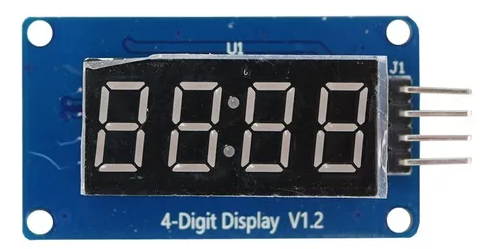
\includegraphics[width=0.5\linewidth]{display.png}
    \caption{Display 7 segmentos 4 digitos}
    \label{fig:enter-label}
\end{figure}

Este display recibe la información utilizando comunicación en serie, con un protocolo propio del fabricante. Para facilitar su uso, este provee una librería que implementa la comunicación y provee funciones simples de usar, tales como \textit{escribir(i: str): bool} y \textit{limpiar()}. Por lo tanto, se implementó el sistema utilizando las funciones provistas para comunicarse, múltiples módulos llaman esas funciones.

En cierto momento el módulo display dejó de funcionar y se lo reemplazó por otro de un fabricante distinto, que funciona con otro protocolo de comunicación. De la misma manera, la empresa provee una librería para utilizar el display. Pero la interfaz no es la misma que la anterior e incluso algunos comportamientos son diferentes. Por ejemplo, en la primer librería el método de escritura devolvía \verb|False| si se quería escribir y ya estaba mostrándose algo en el display, en la nueva si el display esta mostrando algo es pisado al momento de imprimir. Pero, provee un nueva método para verificar que se está mostrando en el momento en que es invocada \verb|get_current(): str|. Entonces para adaptarnos al nuevo display tenemos que modificar todas las llamadas a las viejas funciones al rededor del sistema agregando la lógica nueva.

\begin{figure}[!h]
\caption{Configuración original}
\begin{center}
\begin{tikzpicture}
\umlsimpleclass[]{Cliente}

\umlclass[right=1.5cm of Cliente]{ControlAcme}
{}
{
escribir(i: str): bool  \\
limpiar()
}

\umluniassoc[]{Cliente}{ControlAcme}

\end{tikzpicture}
\end{center}
\end{figure}

\begin{figure}[!h]
\caption{Configuración utilizando la solución de la sección anterior \ref{Accesoalhardware}.}
\begin{center}
\begin{tikzpicture}
\umlsimpleclass[]{Cliente}

\umlclass[right=1.5cm of Cliente]{ControlDisplay}
{}
{
escribir(i: str): bool  \\
limpiar()
}

\umlclass[right=0.5cm of Cliente,below=2cm of Cliente]{ControlAcme}
{}
{
escribir(i: str): bool  \\
limpiar()
}

\umluniassoc[]{Cliente}{ControlDisplay}
\umlinherit[geometry=|-|]{ControlAcme}{ControlDisplay}


\end{tikzpicture}
\end{center}
\end{figure}


Para permitir el cambio propuesto sin tener que realizar todas las modificaciones mencionadas, podemos aplicar el patrón \textit{Adapter}, creando un módulo intermedio con la misma interfaz que \textbf{DisplayLib}.

\begin{figure}[h]
\caption{Configuración nueva}

\begin{center}
\begin{tikzpicture}
\umlsimpleclass[x=-4.5,y=1]{Cliente}

\umlclass[x=0,y=1]{ControlDisplay}
{}
{
escribir(i: str): bool  \\
limpiar()
}
\umlclass[x=-2.5,y=-3]{ControlAcme}
{}
{
escribir(i: str): bool  \\
limpiar()
}
\umlclass[x=2.5,y=-3]{ControlEmca}
{}
{
escribir(i: str): bool  \\
limpiar()
}
\umlclass[x=8,y=0.5]{LibEmca}
{}
{
imprimir(i: str)  \\
get\_current(): str
}
umluniassoc
\umlinherit[geometry=|-|]{ControlAcme}{ControlDisplay}
\umlinherit[geometry=|-|]{ControlEmca}{ControlDisplay}
\umluniassoc[]{Cliente}{ControlDisplay}
\umluniassoc[geometry=-|-]{ControlEmca}{LibEmca}
\end{tikzpicture}
\end{center}
\end{figure}

Por lo tanto el cliente sigue utilizando la misma interfaz para utilizar el display, reduciendo la cantidad y complejidad de los cambios necesarios para utilizar el nuevo display.

Una posible implementación para las funciones \verb|escribir(i: str): bool| y \verb|limpiar()| del módulo \textbf{ControlEmca} es la del código \ref{codigoAdapter}.

\begin{lstlisting}[label={codigoAdapter}, caption=Ejemplo implementación módulo Adapter.]
bool escribir(char* cadena) {
    if (libEmca.get_current() != "") {
        return False;
    }
    libEmca.imprimir(cadena);
    return True;
}

void limpiar() {
    libEmca.imprimir("");
}
\end{lstlisting}

\section{Control en conjunto de dispositivos}
Muchas aplicaciones embebidas robóticas controlan actuadores que deben trabajar en conjunto para lograr el efecto deseado. Por ejemplo, para lograr el movimiento coordinado de un brazo robótico con múltiples articulaciones, todos los motores deben trabajar a la par. De manera similar, el uso de propulsores en una nave espacial en tres dimensiones requiere que muchos de estos dispositivos actúen en el momento preciso y con la cantidad correcta de fuerza para lograr la estabilización de la actitud. En ambos casos existe comunicación entre todos los componentes, ya sea para encadenar la ejecución de ciertos movimientos o para avisar de restricciones. Esto no es tarea simple y requiere de muchas lineas de código, por lo que un diseño orientado al cambio resulta clave.

Como se discutió previamente, en casos como este se puede aplicar la arquitectura de \textit{Control de procesos}. Este hecho no resuelve todos nuestros problemas de diseño, solo nos brinda una guía y un mecanismo de funcionamiento para el sistema. Veamos que estructuras podemos usar para llevar a cabo esta arquitectura de una manera simple y probada (por ejemplo, en el robot desmalezador).

\subsection{Subsistemas de control}

Proponemos al creación de un \textit{subsistema de control} por cada variable a manipular\footnote{Ver tabla conceptos arquitectura Control de Procesos \ref{tab:conceptosArq}} que sea necesaria controlar por el sistema. Como se puede intuir, un subsistema de control se encarga del control de una propiedad en particular y para hacerlo lleva a cabo todas las tareas de la arquitectura a su nivel. Por lo tanto, debe proveer una interfaz que permita setear un valor al que se quiera llevar la propiedad (\textit{setPoint}) y que indique el comienzo de la tarea de control. Un subsistema tiene una estructura similar a la de la arquitectura \ref{fig:arqCtrlRobot}, pero su alcance estará restringido a la variable a manipular y las variables medidas relacionadas.


Veamos ahora de manera mas concreta qué módulos forman parte de cada componente:


\begin{figure}[h]
\caption{Módulos de un subsistema}
\begin{center}
\begin{tikzpicture}

\umlclass[below=6cm of Control]{Sensor}
{}
{setConnection(i: Pipe) \\
signal()
}
\umlnote[below left=-1cm and 1cm of Sensor,width=4cm]{Sensor}{
signal()\{ \\
\ \ \ \ value = getValue()\\
\ \ \ \ pipe.write(value)\\
\}
}

\umlclass[below=3cm of Control]{Actuador}
{}
{actuar()
}
\umlclass[left=2cm of Actuador]{Pipe}
{}
{read(): Measure \\
write(i: Measure)
}


\umlnote[below right=0.5cm and 2cm of Actuador]{Actuador}{
Por lo general se desacopla usando el patrón \textit{command} y su uso puede ser más complejo que solo ejecutar una función.
}

\umlclass[]{Control}
{}
{setPoint(i: Measure)\\
control() \\
connectionRead() \\
setAlgoritmo(i: Algoritmo) \\
setConnection(i: Pipe)
}

\umlclass[above right=-1cm and 2cm of Control]{Algoritmo}
{}
{calcular(): Measure
}
\umlclass[below right=-1.5cm and 2cm of Control]{Data}
{}
{setSetPoint(i: Measure) \\
getSetPoint(): Measure \\
setCurrent(i: Measure) \\
getCurrent(): Measure
}

\umluniaggreg[anchor1=10,anchor2=west]{Control}{Algoritmo}
\umluniaggreg[anchor1=-10,anchor2=west]{Control}{Data}

\end{tikzpicture}
\end{center}
\end{figure}

La manera en la que un \textit{cliente} utiliza el subsistema para lograr que la propiedad que controla vaya al valor que se desea es de la forma indicada en el código \ref{usoSubsistema}.

\begin{lstlisting}[caption=Ejemplo de uso del subsistema.,label={usoSubsistema}]
control.setPoint(valorDeseado)
sensor.signal()
control.connectionRead()
control.control()
\end{lstlisting}

Notar que aparecen un par de módulos que no mencionamos anteriormente, por un lado tenemos \textbf{Algoritmo} el cual se encarga de el calculo necesario para determinar de que manera llamar aplicar un cambio con el/los actuadores. Por ejemplo, determina si se llego o no al \textit{set-point}. Por otro lado, tenemos \textbf{Data} que desacopla el almacenamiento de información relacionada al subsistema. En el caso mas básico solo tenemos el \textit{set-point}, pero puede agregarse todo lo necesario, incluso llevar registro de los valores actuales y pasados.

Ahora, para brindar un comportamiento más complejo, es posible que el control necesite realizar múltiples ciclos para ajustar la variable al valor deseador, como pasa cuando trabajamos con motores paso a paso (luego veremos un ejemplo). ¿Cómo podemos hacer esto usando nuestra estructura? Necesitamos dos modificaciones/adiciones, por un lado, una interrupción de control que llame a cierto método del módulo \textbf{Control} cada determinado tiempo (tiempo del ciclo), generalmente resuelto con una interrupción \textit{temporizada} y por el otro, necesitamos crear la noción de estado a nuestro módulo de control. Tendremos dos estados básico, en espera, cuando no se esta realizando un ciclo de control y trabajando, cuando se haya establecido un \textit{set-point} y se este trabajando para llegar. Para hacerlo utilizamos un nuevo método y el patrón \textit{state} \footnote{La aplicación de este patrón está explicada en la sección \ref{cap:state} Máquinas de estado}.

\begin{figure}[h]
\caption{Estructura módulo \textbf{Control} extendida con estado.}
\begin{center}
\begin{tikzpicture}
\umlclass[x=-4]{Control}
{}
{setPoint()\\
control() \\
cicle() \\
leer() \\
setAlgoritmo(i: Algoritmo) \\
changeState(i: State)
}
\umlnote[x=-5, y=5, width=4cm]{Control}{
Delega al estado interno tanto control() como cicle()
}

\umlclass[x=4, y=3]{State}
{}
{
control() \\
cicle() \\
}

\umlclass[x=2,y=-2]{Waiting}
{}
{
control() \\
cicle() \\
}


\umlclass[x=6,y=-2]{Working}
{}
{
control() \\
cicle() \\
}

\umlinherit[geometry=|-|]{Waiting}{State}
\umlinherit[geometry=|-|]{Working}{State}
\umluniaggreg[geometry=-|-]{Control}{State}

\end{tikzpicture}
\end{center}
\end{figure}

El cliente ejecuta \verb|control()| y la interrupción que marca el ciclo de trabajo ejecuta \verb|cicle()|. De esta manera, cuando el estado es \textit{waiting}, \verb|cicle()| no hace nada y cuando está en \textit{working} \verb|control()| no hace nada y la otra función se encarga de realizar el ciclo de control.
Por supuesto, estas dos funciones son las encargadas de llamar a \verb|changeState()| cuando sea necesario. \verb|control()| cambia a \textit{working} y cuando se alcanza el \textit{set-point}, \verb|cicle()| cambia el estado a \textit{waiting}.

En el diseño del robot desmalezador\cite{paperPomponio} existe un \textit{timer} que desencadena una interrupción cada 1.5\textit{ms} la cual ejecuta el ciclo de control del subsistema de dirección del robot. Este consta de un motor paso a paso, por lo que cada ciclo verifica la diferencia de posición actual con la deseada y si aun no se llego al mínimo de diferencia deseado se envía un pulso al motor para que avance.

Antes de ver un ejemplo repasemos que conseguimos al usar los subsistemas de control. Principalmente encapsulamos el control de cada propiedad de manera independiente, permitiendo que cada una pueda modificarse de manera aislada. Además, se logra que agregar nuevas propiedades con su conjunto de actuadores y sensores conste únicamente en crear nuevos módulos. Se provee una capa de abstracción para construir sobre los sistemas un controlado general (ej. MainController) el cual organizará los esfuerzos de cada uno con el fin de llevar a cabo comportamientos más complejos. Luego veremos como incluso podemos aplicar para esto el patrón \textit{mediator}.

\subsection{Ejemplo}

Veamos como podemos resolver el ejemplo propuesto en el libro de Douglass\cite{douglass} en la sección de 3.4 Mediator Pattern.
\\
\noident
\textbf{Requisitos}
\\
\noident
Se necesita desarrollar el software de control de un brazo robótico que consta de tres actuadores, dos servomotores (uno para rotar y otro para extender o retraer el brazo) y una pinza que se puede cerrar o abrir. Para ello, se provee una función compleja la cual toma coordenadas en el espacio y genera una secuencia de ordenes para que el brazo tome un objeto en la posición determinada por las coordenadas. La secuencia es una serie de pasos, y cada uno consta de una orden para cada actuador del brazo robótico. Estos se deben ejecutar de manera secuencial, es decir que el paso número 2 empezará su ejecución solo si el primero culmino completamente y con éxito. En caso de que las coordenadas sean inalcanzables devuelve 0 pasos. A su vez cada actuador puede informar un error al intentar ejecutar cada movimiento, y si esto pasa se requiere frenar la ejecución total del sistema.

\begin{figure}[h]
\caption{Brazo robótico.}
\begin{centering}
{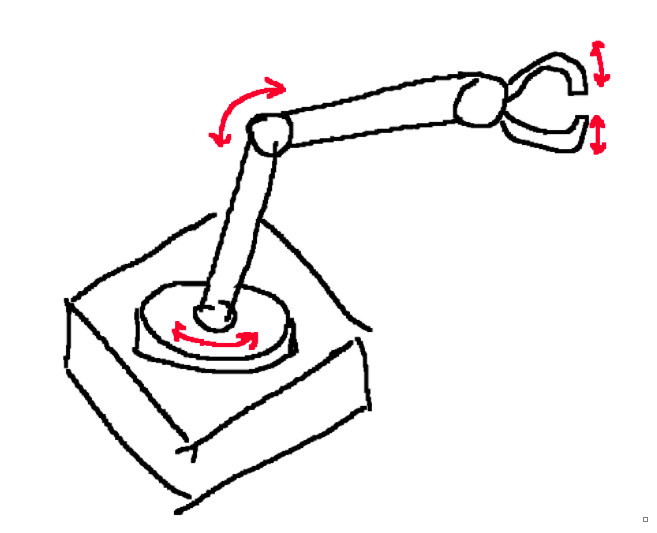
\includegraphics[width=0.5\textwidth]{Screenshot from 2024-08-29 18-44-50.png}\par}
\end{centering}
\end{figure}
\\
\noident
\textbf{Diseño}
\\
\noident
La idea es utilizar el concepto de subsistemas que se introdujo previamente, para ello primero necesitamos identificar las propiedades del mundo físico que debemos controlar. Claramente, lo que se quiere modificar es la posición y el estado de la pinza del brazo, para hacerlo tenemos distintos actuadores que intervienen en diferentes propiedades atómicas. Además, en los requisitos nos especifican que poseemos una función que nos genera una orden para cada actuador. De esta manera definimos un subsistema de control por cada actuador que serán los encargados de llevar a cabo las ordenes generadas. Un ejemplo de orden es rotar 30\textdegree, es claro el \textit{set-point} que se está indicando. Para coordinar los subsistemas proponemos un controlador principal llamado \textbf{MainController}, el cual provee el método \verb|graspAt(i: Coordenadas)| al cliente, realiza la generación de los pasos y controla su ejecución. La estructura seria algo así:


\begin{figure}[h]
\caption{Diagrama componentes sistema brazo}
\begin{center}
\begin{tikzpicture}
\umlsimpleclass[]{MainController}

\umlsimpleclass[x=-5]{Cliente}

\umlsimpleclass[x=-5, y=-3]{SubSistemaRotor}

\umlsimpleclass[x=0, y=-3]{SubSistemaExtensor}

\umlsimpleclass[x=5, y=-3]{SubSistemaPinza}

\umluniassoc{Cliente}{MainController}
\umluniassoc[anchor1=-160, anchor2=60]{MainController}{SubSistemaRotor}
\umluniassoc[anchor1=-80, anchor2=70]{MainController}{SubSistemaExtensor}
\umluniassoc[anchor1=-10, anchor2=70]{MainController}{SubSistemaPinza}
\umluniassoc[anchor1=110, anchor2=-170]{SubSistemaRotor}{MainController}
\umluniassoc[anchor1=110, anchor2=-100]{SubSistemaExtensor}{MainController}
\umluniassoc[anchor1=110, anchor2=-20]{SubSistemaPinza}{MainController}
\end{tikzpicture}
\end{center}
\end{figure}
(Añadir al gráfico que significa cada flecha, control(), notifyEnd() y onError())

Podemos pensar que el gráfico tiene cierta similaridad conceptual con el patrón \textit{mediator}, donde tenemos un módulo \textbf{Mediator} que coordina el trabajo de los \textbf{College} en este caso los subsistemas. Gamma indica que el patrón suele ser apropiado para casos en lo que se tiene un conjunto de objetos que se comunican de manera compleja pero fija. En este caso la comunicación no es tan compleja, pero puede considerarse lo suficiente como para implementar el patrón. En particular, el \textbf{MainController} indica los \textit{set-point} de cada subsistema y desencadena el proceso de control en cada uno. Y viceversa, los subsistemas indican cuando llegan al \textit{set-point} o cuando se encuentran un error. A su vez, los subsistemas no se comunican de manera directa entre si, todo pasa por el \textbf{MainController}.

Veamos en detalle los módulos conforman cada componente comenzando por los módulos básicos que debemos crear para representar el hardware dado (ver grafico \ref{estructuraActuadores}):

\begin{figure}[h]
\label{estructuraActuadores}
\caption{Actuadores paso a paso.}
\begin{center}
\begin{tikzpicture}
\umlclass[]{StepDevice}
{}
{
right() \\
left() \\
disable()\\
enable() \\
pulse()
}

\umlclass[below left=1cm and -0.3cm of StepDevice]{Rotor}
{}
{
right() \\
left() \\
disable() \\
enable() \\
pulse()
}

\umlclass[below right=1cm and -0.3cm of StepDevice]{Extensor}
{}
{
right() \\
left() \\
disable()\\
enable() \\
pulse()
}

\umlinherit[geometry=|-|]{Rotor}{StepDevice}
\umlinherit[geometry=|-|]{Extensor}{StepDevice}

\end{tikzpicture}
\end{center}
\end{figure}

Estos son motores paso a paso \footnote{Se utiliza el mismo diseño propuesto para el robot desmalezador\cite{paperPomponio}.}, lo cuales para controlarlos debemos primero setear su dirección llamando a las funciones \verb|right| o \verb|left| para luego avanzar un paso llamando al método \verb|pulse|. Claramente para que lleguen a la posición deseada puede ser necesario invocar reiteradas veces al método \verb|pulse|. Esto será importante a la hora de diseñar el subsistema que controlará cada dispositivo.

En cambio, en el caso de la pinza se utiliza un dispositivo que tiene dos estados, abierto o cerrado, por lo que solo tenemos dos funciones para cambiar entre los estados.

\begin{figure}[h]
\caption{Interfaz módulo Pinza.}
\begin{center}
\begin{tikzpicture}
\umlclass[]{Pinza}
{}
{
abrir() \\
cerrar()
}

\end{tikzpicture}
\end{center}
\end{figure}

Vemos ahora los sensores asociados a cada actuador, estos heredaran del módulo sensor pasivo el cual provee dos funciones, \verb|setConnection(i: Pipe)| la cual configura el \textbf{Pipe} por el cual se enviará la información obtenida del sensor cuando la otra funciones, \verb|signal()| sea invocada.

\begin{figure}[h]
\caption{Sensores}
\begin{center}
\begin{tikzpicture}
\umlclass[]{PasiveSensor}
{}
{
setConnection(i: Pipe) \\
signal() \\
}

\umlclass[x=-5,y=-4]{SensorEstadoPinza}
{}
{
setConnection(i: Pipe) \\
signal() \\
}

\umlclass[x=0,y=-4]{SensorPosRotor}
{}
{
setConnection(i: Pipe) \\
signal() \\
}

\umlclass[x=5,y=-4]{SensorPosExtensor}
{}
{
setConnection(i: Pipe) \\
signal() \\
}

\umlinherit[geometry=|-|]{SensorEstadoPinza}{PasiveSensor}
\umlinherit[geometry=--]{SensorPosRotor}{PasiveSensor}
\umlinherit[geometry=|-|]{SensorPosExtensor}{PasiveSensor}


\end{tikzpicture}
\end{center}
\end{figure}

Para completar los módulos que conforman a un subsistema de control nos falta mostrar como se define el \textbf{Controller}. Vamos a diferenciar dos tipos de \textbf{Controllers}, uno para los sensores que requieren un control durante un determinado lapso de tiempo para poder llegar a su \textit{set-point} y los que no. En este ejemplo, tenemos dos motores paso a paso que representan el primer tipo y la pinza que corresponde al segundo. Vemos primero el caso más ``complejo'', como el proceso de control se extiende en el tiempo necesitamos añadir al sistema un mecanismo por el cual cada cierto intervalo ejecute un ciclo de control, es decir, lea la posición actual, decida y actúe. Para eso, en el diseño del robot desmalezador se propuso la creación de una interrupción temporizada, la cual se ejecuta cada 1.5\textit{ms} y desencadena el control de los subestimas necesarios.


\begin{figure}[h]
\caption{Timer}
\begin{center}
\begin{tikzpicture}
\umlclass[]{Timer}
{}
{
setPeriod(i: Real) \\
start() \\
stop() \\
tickHandler()
}

\umlnote[above right=-2cm and 1cm of Timer,width=7cm]{Timer}{
tickHandler() \{ \\
subsistemControlTimeout.execute() \\
\}
}

\umlsimpleclass[below right=0cm and 2cm of Timer]{Command}
\umluniassoc[geometry=|-]{Timer}{Command}
\end{tikzpicture}
\end{center}
\end{figure}

El método \verb|tickHandler()| ejecutará \textit{Commands} por cada subsistema que lo necesite, por lo tanto se iniciará en cada uno el ciclo de control. En particular, la orden la usamos para desacoplar como es invocado el inicio del \textbf{Timer}.

Una vez solucionada la invocación, tenemos que introducir un nuevo módulo que será usado en el \textbf{Controller}. Ahora, tenemos dos modos de operación de este ultimo, cuando no se está trabajando y cuando si. Dependiendo de cual de los dos esté activo el comportamiento será diferente, ya que por ejemplo, no apagamos el \textbf{Timer} cuando no se está haciendo un movimiento, sino que cuando este desencadene la ejecución del ciclo el \textbf{Controller} ignorará la orden. Para esto hacemos uso del patrón \textit{State} de Gamma[\cite{Gamma:1995:DPE:186897}, el cual está explicado en la sección \ref{cap:state}. En particular, el \textbf{Controller} delegará dos funciones de su interfaz al \textit{state}, \verb|control()| y \verb|move()| (luego lo veremos en más detalle).

\begin{figure}[h]
\caption{Módulos necesarios para complementar el Controller}
\begin{center}
\begin{tikzpicture}
\umlclass[]{OperationState}
{}
{
control(i: Controller) \\
move(i: Controller) \\
}

\umlclass[x=-3,y=-4]{Moving}
{}
{
control(i: Controller) \\
move(i: Controller) \\
}

\umlclass[x=3,y=-4]{Waiting}
{}
{
control(i: Controller) \\
move(i: Controller) \\
}

\umlinherit[geometry=|-|]{Moving}{OperationState}
\umlinherit[geometry=|-|]{Waiting}{OperationState}

\end{tikzpicture}
\end{center}
\end{figure}

Siguiendo con la guía de creación de subsistemas, también debemos definir el módulo \textbf{Data} que almacena la información utilizada por el mismo y el módulo \textbf{Algoritmo} que encapsula los cálculos necesarios para determinar que cambio aplicar.

\begin{figure}[h]
\caption{Módulos complementarios a Controller.}
\begin{center}
\begin{tikzpicture}
\umlclass[x=-3]{Data}
{}
{
setSetPoint(i: Measure) \\
getSetPoint(): Measure \\
setCurrent(i: Measure) \\
getCurrent(): Measure
}

\umlclass[x=3]{Algoritmo}
{}
{
compute(i: Data): Measure
}

\end{tikzpicture}
\end{center}
\end{figure}

Ahora si tenemos todos los módulos necesarios para mostrar nuestro \textbf{Controller}.

\begin{figure}[h]
\caption{Controller}
\begin{center}
\begin{tikzpicture}
\umlclass[]{Controller}
{}
{
setConnection(i: Pipe) \\
readConnection() \\
setSetPoint(i: Measure) \\
getData(): Data \\
getAlgoritmo(): Algoritmo \\
changeOperationState(i: OperationState) \\
move() \\
control()
}

\umlsimpleclass[above right=-1.5cm and 1cm of Controller]{Data}
\umlsimpleclass[above right=-2.5cm and 1cm of Controller]{Algoritmo}
\umlsimpleclass[above right=-3.5cm and 1cm of Controller]{OperationState}
\umlsimpleclass[above right=-4.5cm and 1cm of Controller]{Pipe}

\umluniaggreg[anchor1=22,anchor2=west]{Controller}{Data}
\umluniaggreg[anchor1=7,anchor2=west]{Controller}{Algoritmo}
\umluniaggreg[anchor1=-7,anchor2=west]{Controller}{OperationState}
\umluniaggreg[anchor1=-22,anchor2=west]{Controller}{Pipe}

\end{tikzpicture}
\end{center}
\end{figure}

Veamos la funcionalidad de cada método que provee la interfaz de Controller:
\begin{itemize}
    \item setConnection: configura el tubo por el cual llegará la información proveniente de el/los sensores.
    \item readConnection: lee del pipe y almacenar la información en el módulo data.
    \item setSetPoint: se utiliza antes de comenzar el control para configurar el valor al que se quiere llegar.
    \item getData: devuelve el objeto Data asociado al \textbf{Controller}.
    \item getAlgoritmo: lo mismo que con Data.
    \item changeOperationState: cambia el estado del modo de operación, en la configuración básica las transiciones posibles son de \textit{Waiting} a \textit{Moving} y viceversa.
    \item move: es el método ejecutado en cada timeout del \textbf{Timer} de control, realiza un paso del ciclo de control si el estado es \textit{Moving}.
    \item control: se utiliza para comenzar el ciclo de control, es el puntapié inicial que desencadena el comportamiento de todo el subsistema.
\end{itemize}

Imaginemos que un cliente quiere utilizar el subsistema, qué métodos tiene que ejecutar si ya está configurado? Primero debe indicarle a los sensores que escriban el valor de lectura en el pipe, para esto hay que ejecutar el método \verb|signal| en cada uno. Luego el \textbf{Controller} debe leer esta información del pipe y almacenarla, para esto ejecutamos \verb|readConnection|. Ahora, seteamos el setPoint deseado y por ultimo ejecutamos \verb|control|, la cual tomará los valores actuales, el \textit{set-point} y decidirá utilizando el módulo \textbf{Algoritmo} que cambio realizar en los actuadores. En el caso del \textbf{Rotor}, por ejemplo, podrá tanto cambiar la dirección de giro, como avanzar un paso ejecutando \verb|pulse()|. Un ejemplo del metodo \verb|control()| para el caso del subsistema del \textbf{Rotor} y estado de operación \textit{Waiting}, puede ser la del código \ref{impControl} (recordar que el \textit{set-point} del subsistema del rotor es una medida en grados).

\begin{lstlisting}[caption=Ejemplo implementación control,label={impControl}]
    void control(Controller controller) {
        setPoint = data.getSetPoint();
        current = data.getCurrent();
        dif = controller.algoritmo.calculate()
        if abs(dif) > LIMIT_ACCEPT && dif > 0 {
            rotor.left();
            rotor.pulse;
            controller.changeOperationState(moving);
            return;
        }
        if abs(dif) > LIMIT_ACCEPT && dif < 0 {
            rotor.right();
            rotor.pulse;
            controller.changeOperationState(moving);
            return;
        }
    }
\end{lstlisting}

El método \verb|move| tendrá un comportamiento similar pero en el aso de cambiar de estado lo hará a \textit{Waiting}. Para el caso de la \textbf{Pinza}, el \textbf{Controller} es más simple ya que no necesitamos los estados, pero el uso y comportamiento es similar. Por lo que para este ejemplo, vamos a necesitar crear dos subsistemas con estados y uno sin.

Ya tenemos los subsistemas, por lo que siguiendo con nuestro diagrama, nos falta la parte del \textbf{MainController}. El cual sera el encargado de brindar una interfaz al cliente y a su vez coordinar cada subsistema. Recordando los requerimientos, sabemos que tenemos una función que generar una secuencia de pasos donde cada uno implica una acción sobre los tres actuadores. ¿Cómo podemos diseñar este comportamiento? Se me ocurre usar un \textit{iterator} para recorrer los pasos y usar el patrón \textit{command} para cada uno. En particular, aplicaremos una de las modificaciones del patrón mencionada por Gamma\cite{Gamma:1995:DPE:186897}, en donde una orden al ser ejecutada desencadena una ejecución del resto de las ordenes. Veamoslo en los gráficos \ref{iterator} y \ref{orden}.


\begin{figure}[h]
\caption{Iterator}
\label{iterator}
\begin{center}
\begin{tikzpicture}
\umlclass[]{Steps}
{}
{
primero() \\
siguiente()\\
elementoActual(): Orden\\
haTerminado(): Bool\\
}


\end{tikzpicture}
\end{center}
\end{figure}

\begin{figure}[h]
\caption{Orden}
\label{orden}
\begin{center}
\scalebox{.75}{
\begin{tikzpicture}

\umlclass[]{Orden}
{}
{
ejecutar()
}

\umlclass[below left=2cm and 4.5cm of Orden]{OrdenRotor}
{
OrdenRotor(i: Measure)
}
{
ejecutar()
}

\umlclass[below left=2cm and -1cm of Orden]{OrdenExtensor}
{
OrdenExtensor(i: Measure)
}
{
ejecutar()
}

\umlclass[below right=2cm and -1cm of Orden]{OrdenPinza}
{
OrdenPinza(i: Measure)
}
{
ejecutar()
}

\umlclass[below right=2cm and 4cm of Orden]{OrdenMultiple}
{
OrdenMultiple(i: OrdenRotor, \\ i: OrdenExtensor, \\i: OrdenPinza)

}
{
ejecutar()
}
\umlinherit[geometry=|-|]{OrdenRotor}{Orden}
\umlinherit[geometry=|-|]{OrdenExtensor}{Orden}
\umlinherit[geometry=|-|]{OrdenPinza}{Orden}
\umlinherit[geometry=|-|,arm1=2.54cm]{OrdenMultiple}{Orden}
\umluniaggreg[geometry=-|-, anchor1=east, arm1=1cm]{OrdenMultiple}{Orden}
\umlnote[above=4cm of OrdenMultiple,width=5cm]{OrdenMultiple}{
ejecutar() \{  \\
\ \ \ \ ordenRotor.ejecutar() \\
\ \ \ \ ordenExtensor.ejecutar() \\
\ \ \ \ ordenPinza.ejecutar() \\
\}
}

\end{tikzpicture}}
\end{center}
\end{figure}

\begin{figure}
\begin{lstlisting}[caption=Ejemplo OrdenRotor]
void ejecutar {
    rotorController.setSetPoint(setPoint)
    rotorSensor.signal()
    rotorController.readConnection()
    rotorController.control()
}
\end{lstlisting}
\end{figure}

Tenemos un iterado de ordenes, en particular múltiples, que almacena todos los pasos de ejecución que la función provista generará. Por lo que el \textit{MainController} podrá recorrerlos ejecutando cada orden de manera sencilla. Logramos, almacenar el procedimiento a realizar y desacoplar como se pone en marcha el ciclo de control en cada subsistema.

\begin{figure}[h]
\caption{MainController}
\begin{center}
\scalebox{.75}{
\begin{tikzpicture}
\umlclass[x=-5,y=0]{MainController}
{
MainContoller(i: StepsComputator)
}
{
graspAt(i: Coordenadas) \\
notifyReady() \\
notifyError() \\
changeState()
}
\umlclass[x=0,y=-4]{MainControllerState}
{}
{
graspAt(i: Coordenadas) \\
notifyReady(i: MainCtrl) \\
}
\umlclass[x=-10,y=-8]{MainWaiting}
{}
{
graspAt(i: Coordenadas) \\
notifyReady(i: MainCtrl) \\
}
\umlclass[x=-5,y=-8]{Main0}
{}
{
graspAt(i: Coordenadas) \\
notifyReady(i: MainCtrl) \\
}
\umlclass[x=0,y=-8]{Main1}
{}
{
graspAt(i: Coordenadas) \\
notifyReady(i: MainCtrl) \\
}
\umlclass[x=5,y=-8]{Main2}
{}
{
graspAt(i: Coordenadas) \\
notifyReady(i: MainCtrl) \\
}



\umlclass[x=3,y=0]{StepsComputator}
{
}
{
geneararStepts(i: Coordenadas) \\
}
\umluniaggreg{MainController}{StepsComputator}
\umluniaggreg[geometry=|-]{MainController}{MainControllerState}
\umlinherit[geometry=|-|]{MainWaiting}{MainControllerState}
\umlinherit[geometry=|-|]{Main0}{MainControllerState}
\umlinherit[geometry=|-|]{Main1}{MainControllerState}
\umlinherit[geometry=|-|]{Main2}{MainControllerState}
\umlnote[x=-9,y=-4,width=6.5cm]{MainController}
{
void notifyReady() \{ \\
\ \ \ \ mainControllerState.notifyReady() \\
\}
}


\end{tikzpicture}
}
\end{center}
\end{figure}

Hasta la introducción de \textbf{MainController} todo lo que estábamos haciendo era solo seguir con el concepto de subsistemas. Pero para poder cumplir los requerimientos particulares del ejemplo, necesitamos introducir ciertos cambios. Como necesitamos ejecutar un paso a la vez, tenemos que esperar que todas las ordenes que enviamos en el paso anterior a los subsistemas. Para ello hacemos uso del patrón \textit{state}, al cual delegaremos las funciones \verb|graspAt| y \verb|notifyReady|. La idea es cambiar el comportamiento de estas dependiendo de en qué estadio estamos, seguiremos el siguiente gráfico \ref{statesMainController}.

\begin{figure}[h]
\label{statesMainController}
\caption{Transiciones de estados del MainController}
\begin{center}
\begin{tikzpicture}

\umlsimpleclass[x=-2]{Waiting}
\umlsimpleclass[x=2]{0}
\umlsimpleclass[x=2, y=-2]{1}
\umlsimpleclass[x=2, y=-4]{2}

\umltrans[arg=graspAt,pos=0.5]{Waiting}{0}
\umltrans[arg=notifyEnd,pos=0.5]{0}{1}
\umltrans[arg=notifyEnd,pos=0.5]{1}{2}
\umltrans[arg=notifyEnd,pos=1.5,arm1=3cm,geometry=-|-]{2}{0}

\end{tikzpicture}
\end{center}
\end{figure}

Por lo que, el estado Waiting no implementa \verb|notifyOrder| y a su vez 0, 1 y 2 no implementan \verb|graspAt|. En cambio, Waitating implementan \verb|graspAt| la cual computa los pasos y ejecuta el primero utilizando el iterator. Luego, por cada \verb|notifyEnd| los subsistemas le avisan al MainController que terminaron la orden y por cada una transaccionamos a un estado nuevo. Luego de que se ejecuta \verb|graspAt| se transiciona al estado 0 en el cual al recibir un \verb|notifyEnd| se transiciona a 1 y lo mismo hasta llegar a 2. En cambio, cuando estamos en el estado 2 y se ejecuta \verb|notifyEnd| lo que se hará es ejecutar un nuevo paso si en el iterador de pasos quedan pasos, en caso contrario se transicionará a Waiting ya que se terminó la ejecución. Está claro que para poder llevar a cabo este comportamiento es necesario que los subsistemas respondan a las necesidades. Por lo que cada uno tendrá que llamar al método \verb|notifyEnd| del \textbf{MainController} cuando efectivamente terminen la ejecución de la orden, es decir, el ciclo de control. Para hacerlo se puede agregar la llamada en la cuando se decide transicionar de \textit{Moving} a \textit{Waiting }o en el caso de los subsistemas sin estados, luego de aplicar los cambios en los actuadores.

\newpage
\section{Obtención de información}

Generalmente una tarea importante que tienen los sistemas embebidos es recavar información proveniente de sensores. Existen diferentes formas en las que los sensores transmiten información al sistema, algunos, por ejemplo un sensor de temperatura, setea en el pin en el que esta conectado un cierto valor de tensión, por lo que el sistema solo debe consultar el valor del pin. Otros, en cambio, se comunican mediante interrupciones, por ejemplo un sensor de efecto \textbf{Hall} genera una interrupción por cada detección de campo magnético. Por lo tanto, si lo estamos usando para calcular las \textbf{RPM} de cierto componente giratorio, debemos llevar una cuenta de las interrupciones que generó en cierto periodo de tiempo y realizar cierta matemática. Evidentemente, es necesario que alguna porción de nuestro sistema se encargue de hacerlo y maneje las interrupciones generadas por el sensor. Algo similar pasa con otro tipos de sensores como joysticks, botones, etc. Es por esto que resulta útil una forma general de atacar este problema, en el diseño del robot desmalezador, Laura utilizo una estructura de módulos que lleva a cabo las actividades necesarias para integrar al sistema los sensores que generan interrupciones.

\begin{figure}[h!]
\caption{Componente sensor activo.}
\centering
\begin{tikzpicture}\hypertarget{fig:ConnectBufferToMCU}{}
%-------------Estilos para dibujar-----
\tikzstyle{módulo}=[minimum width=1cm,inner sep=2mm,above right,draw,align=center,minimum width=2cm, font=\bfseries]

\tikzstyle{supest}=[rounded corners=1.5mm, minimum width=2cm,inner sep=2mm,draw,text width=2cm]

\tikzstyle{componente}=[minimum width=2cm,inner sep=2mm,draw,text width=2cm]

\tikzstyle{nombre}=[inner sep=0mm, font=\bfseries]

\tikzstyle{pipe}=[-latex,thick,line width=4pt]

\tikzstyle{modExt}=[minimum width=1cm,inner sep=2mm,above right,draw, dotted,line width=2pt,align=center,minimum width=2cm,color=gray, font=\bfseries]

\tikzstyle{flechaFisica}=[-latex,snake=coil,segment aspect=0, red, thick];
%--------------------------


\node[módulo, below =4cm of CR](Pin){Pin};

\node[módulo, above left=0.5cm and 2cm of Pin](CountTime){Count};

\draw[flechaFisica](Pin) -| (CountTime);

\node[módulo, above=1cm of CountTime](CRpinCollector){Collector};

\draw[-latex](CountTime) edge (CRpinCollector);

\node[módulo, left=1cm of CRpinCollector](CRBuffer){Buffer};

\draw[-latex](CRBuffer) edge (CRpinCollector);

\node[módulo, below=5cm of CRBuffer](BufferReader){Cliente};

\draw[-latex](BufferReader) edge (CRBuffer);

\node[nombre, below right = 1cm and -3cm of Pin](ConnectBufferToMCU){};

\node[componente, fit=(Pin)(CountTime)(CRBuffer)(ConnectBufferToMCU)]{};

%%------------------------------Referencias------------

\node[módulo, below left=1cm and -0.5cm of BufferReader](mod){nombre};
\node[right =0.5cm of mod](modDesc){módulo};

\node[right=4cm of modDesc](x1){};
\node[right=2cm of x1](x2){};
\draw[-latex](x1)--(x2);
\node[right=0.3cm of x2](llp){llamada a procedimiento};

\node[below=0.5cm of mod.south west](x1a){};
\node[below=0.5cm of mod.south east](x2a){};
\draw[flechaFisica](x1a)--(x2a);
\node[below right=-0.4cm and 0.3cm of x2a, text width=4cm](hand){llamada a procedimiento a partir de una interrupción física (handler)};

\node[below=0.7cm of x1](x1b){};
\node[below=0.7cm of x2](x2b){};
\draw[dashed](x1b)--(x2b);
\node[right=0.3cm of x2b](rf){conexión física};
%
\node[supest, fit=(mod)(hand)(llp)]{};

\end{tikzpicture}
\label{fig:ConnectBufferToMCU}
\end{figure}



Podemos distinguir 4 módulos principales, \textbf{Pin} que es la representación en el diseño del hardware asociado al dispositivo que genera e introduce la interrupción, esta es manejada por \textbf{Count} que es un módulo perteneciente al patrón \textit{Command} el cual cumple la función de comando para reemplazar la utilización de \textit{callbacks}. En particular, opera sobre \textbf{Collector} almacenando en este la información relevante del evento (interrupción). Esta por lo general es un \textit{timestamp} y la cantidad de veces que sucedió.  Por ultimo, \textbf{Buffer} actúa como buffer de la información recibida a través, posee un método que permite obtener el valor recibido. Cuando es invocada toma los valores necesarios que se almacenan en el \textbf{Collector} y realiza los cómputos necesarios para calcular el dato pedido.

Veamos esta estructura más en detalle con un ejemplo de aplicación. Supongamos que tenemos un sensor \textit{Hall} montado en una rueda y con este queremos medir la velocidad a la que se está moviendo. Por lo tanto, cada vez que el sensor detecte un campo magnético emitirá una interrupción que será manejada por el módulo \textbf{Count} que es un comando, por lo que sabe que funciones ejecutar del módulo \textbf{Collector}. \textbf{Count} tiene la siguiente interfaz:
\begin{itemize}
    \item execute() registra en el acumulador el instante actual, mediante Collector::currentTime, y luego incrementa el contador de interrupciones invocando Collector::addOne.
\end{itemize}

Y la de el módulo \textbf{Collector}:
\begin{itemize}
    \item currentTime(): registra internamente el momento actual de cuando el método es invocado.
    \item getCurrentTime(): devuelve el último instante de tiempo registrado por el módulo.
    \item addOne(): incrementa el contador interno que cuenta las ocurrencias de interrupción del sensor \textit{Hall}.
    \item total(): retorna el valor del contador interno.
\end{itemize}

Por lo tanto cuando se pida el valor de velocidad al \textbf{Buffer} este llamará a las funciones necesarias del \textbf{Collector} para obtener información, computará el valor y lo retornará.

De esta forma un cliente de nuestro componente puede obtener la información recibida a través del pin sin necesidad de manejar las interrupciones y todas las operaciones asociadas al tratamiento de los datos.

Por ejemplo, si tenemos un sensor de efecto Hall que emite una interrupción en cada detección del campo magnético y lo usamos para medir la velocidad de una rueda, podemos utilizar el siguiente diseño (obviamente, aplicando lo que acabamos de ver):

\begin{figure}[H]
\caption{Ejemplo}
\begin{center}
\scalebox{.90}{
\begin{tikzpicture}

\umlclass[]{HallSensor}
{}
{
start() \\
stopt() \\
signalHandler() \\
setCommand(i: Command)
}

\umlnote[above left=1cm and -1cm of HallSensor,width=3cm]{HallSensor}
{
signalHandler() \{\\
\ \ \ \ cmd.execute() \\
\}
}

\umlclass[right=2cm of HallSensor]{Count}
{}
{
execute() \\
}

\umlnote[above=1cm of Count,width=4cm]{Count}
{
Hereda de Command \\
execute() \{ \\
\ \ \ coll.currentTime() \\
\ \ \ coll.addOne() \\
\}
}

\umlclass[below=1cm of HallSensor]{Collector}
{}
{
currentTime() \\
getCurrentTime(): Real \\
addOne() \\
preSum(): int \\
total(): int \\
periodTime(): Real \\
initPeriod()\\
}

\umlclass[right=2cm of Collector]{Buffer}
{
Buffer(i: Collector)
}
{
setConnection(i: Pipe) \\
signal() \\
}

\umlnote[below left=1.5cm and -4cm of Buffer,width=7.5cm]{Buffer}
{
signal() \{ \\
\ \ vColl.initPeriod() \\
\ \ t = vColl.periodTime()\\
\ \ nInterrup = vColl.preSum()\\
\ \ velRPM = func(t,NINTERRUP,DELTAT)\\
\ \ pipe.write(velRPM)\\
\} \\

DELTAT y NINTERRUP son constantes
}

\umlnote[left=1cm of Collector,width=4cm]{Collector}
{
addOne() \{ \\
\ \ nbr++ \}\\
\\
currentTime()\{\\
\ \ coll.currentTime()\\
\ \ if nbr == 0\\
\ \ \ \ initialT = coll.getCurrentTime()\\
\}\\
\\
getCurrentTime()\{\\
\ \ coll.getCurrentTime() \}
\\
\\
preSum()\{\\
\ \ return preN \}\\
\\
total()\{\\
\ \ return totalN \}\\
\\
periodTime()\{\\
\ \ return periodT \}\\
}

\umluniaggreg{Buffer}{Collector}
\umluniaggreg{HallSensor}{Count}

\end{tikzpicture}
}
\end{center}
\end{figure}


\textbf{Periodicidad}

Algunos sistemas se encargan de mostrar, almacenar o verificar información de sensores cada cierto tiempo. No resulta crítico perder valores intermedios, es decir que no nos interesa una respuesta inmediata. Un ejemplo puede ser una estación meteorológica o un dispositivo médico de control como un tensiómetro que registra los valores de presión del paciente cada cierto periodo de tiempo.

Una implementación intuitiva es escribir un \textit{loop} y en el que verificamos la información de los sensores y luego ejecutamos una función \textit{sleep} que bloquea la ejecución determinada cantidad de tiempo. Esto tiene varias desventajas, primero el tiempo de ejecución de nuestra rutina alarga el periodo, si queremos agregar otras funcionalidades a realizar mientras esperamos el periodo tendríamos que dividir el \textit{sleep} y calcular tiempo de ejecución.

Una solución que nos parece más adecuada desde el punto de vista del diseño orientado al cambio es la siguiente. Se registra un temporizador que cada \textit{x} cantidad de tiempo gatilla una interrupción, esto es provisto por muchos entornos de desarrollo para sistemas embebidos como \textit{Arduino}.
Registraremos un \textit{handler} para esta que será un módulo orden del patrón  \textit{Command} el cual encapsula que funciones son necesarias ejecutar para llevar a cabo la funcionalidad deseada. Por ejemplo, pedir la información de los sensores, ya sea a sus respectivos \textbf{Buffers} (si tenemos sensores como en el ejemplo anterior) o a los sensores en si, si son de otro tipo y luego registrarla en cierta módulo (que oculte una estructura de datos). De esta forma liberamos el procesador en los tiempos de espera y desacoplamos esta funcionalidad.



\section{Control anti-rebote}
Muchos dispositivos de entrada para sistemas embebidos utilizan contacto metal con metal para indicar eventos de interés, como botones, interruptores y relés. A medida que el metal entra en contacto, se produce una deformación física que resulta en un contacto intermitente de las superficies. Esto genera señales que de no ser filtradas pueden causar una lectura errónea. 

En la bibliografía encontramos una propuesta de solución que desde mi punto de vista está más cerca de la implementación que del diseño. Esta consiste en utilizar un temporizador para dar un tiempo de gracia antes de confirmar una transición en el estado. Esto es, al percibir un cambio en la entrada se inicia el \textit{timer} y se confirma el cambio de estado solo si el valor de la entrada sigue siendo distinto que antes de percibir la modificación. 

\begin{lstlisting}[caption=Código ejemplo]
void ButtonDriver_eventReceive(ButtonDriver* const me) {
    Timer_delay(me->itsTimer, DEBOUNCE_TIME);
    if (Button_getState(me->itsButton) != me->oldState) {
        /* must be a valid button event */
        
        me->oldState = me->itsButton->deviceState;
        
        if (!me->oldState) {
            
            /* must be a button release, so update toggle value */
            if (me->toggleOn) {
                me->toggleOn = 0; /* toggle it off */
                Button_backlight(me->itsButton, 0);
                MicrowaveEmitter_stopEmitting(me->itsMicrowaveEmitter);
            }
            else {
                me->toggleOn = 1; /* toggle it on */
                Button_backlight(me->itsButton, 1);
                MicrowaveEmitter_startEmitting(me->itsMicrowaveEmitter);
            }
        }
        /* if it’s not a button release, then it must
        be a button push, which we ignore.
        */
    }
}
\end{lstlisting}

Desde el punto de vista de la IS, creo que se están combinando múltiples responsabilidades en un mismo módulo, lo cual no ayuda a lograr el objetivo de diseñar para el cambio. El estado y la decisión de transicionar son responsabilidad de un módulo, lo que puede generar inconvenientes si se quiere cambiar el criterio de aceptación de la señal, por ejemplo. Esto se evidencia en el código ejemplo del libro de Douglass donde tenemos múltiples sentencias \textit{if} anidadas. Una solución que se ajusta más a nuestros principios involucraría el patrón \textit{State} de Gamma y otro módulo que cumpla la función de verificar el cambio.

Parece ser un problema vigente, se habla mucho en internet sobre eso, por ejemplo \textit{A Guide to Debouncing} de Jack G. Ganssle.


\section{Manejo de interrupciones}
Algunos microcontroladores como \textbf{Arduino} proveen en su entorno de desarrollo herramientas para manejar interrupciones. En particular, permiten asociar un método (\textit{handler}) a un cierto evento por ejemplo un cambio en un pin digital.

\section{Máquinas de estado}\label{cap:state}


Muchos sistemas ajustan su comportamiento durante la ejecución en base a diferentes causas como interacciones externas, su propios requerimientos, etc. Por ejemplo, el sistema de control de un microondas no iniciará el calentamiento si la puerta está abierta, es decir que existe un estado interno en el que el microondas está al tener la puerta abierta y no permite cierto comportamiento que en otro estado si seria posible. De manera similar, podemos pensar que algunas partes de los sistemas responden a diferentes estados. Un ejemplo sería la dirección de giro de un motor en un robot, que podría representarse como un estado: si el motor está en un estado de "girar hacia adelante" o "girar hacia atrás", su comportamiento cambia en consecuencia. Además, si el sistema está llevando a cabo una operación, su estado podría ser \textit{trabajando}, y al finalizar, podría retornar al estado \textit{esperando}, lo que también modificaría su comportamiento. Otro ejemplo es un sistema de climatización: el estado del termostato podría ser \textit{calentando} o \textit{enfriando}, dependiendo de lo configurado por el usuario. Por lo tanto, es común enfrentarse a la gestión de estados, transiciones y todos los cambios en el comportamiento que resultan de estos.

Una solución de implementación intuitiva para aplicar estados es almacenarlos en una variable y verificar esta última para cambiar el comportamiento de las funciones. Por ejemplo:

\begin{lstlisting}
calentar() {
    if (estado == PuertaAbierta) {
        return
    } else {
        magnetron.encender()
    }
}
\end{lstlisting}

Este enfoque de es una solución directa. Sin embargo, presenta algunas desventajas cuando se desea modificar o extender el código. Por ejemplo, si se necesita agregar nuevos estados o cambiar el comportamiento del sistema, este método puede volverse rápidamente difícil de gestionar. Una de las principales desventajas es la complejidad creciente. A medida que se agregan más estados, cada función requerirá más verificaciones de estado, lo que llevará a una proliferación de estructuras \textit{if-else} o \textit{switch-case}. Esto no solo hace que el código sea más difícil de leer, sino que también aumenta la probabilidad de errores, ya que cada nuevo estado debe ser cuidadosamente incorporado en todas las partes relevantes del sistema. Además, este enfoque dificulta la sostenibilidad, cuando el comportamiento de un estado debe cambiar, es posible que se necesiten modificaciones en varias funciones. Esto puede resultar en código duplicado, o incluso puede ser difícil saber que modificar, lo que complica el proceso de realizar cambios sin introducir errores. Otra desventaja es la poca modularidad, no es claro el comportamiento asociado a cada estado. Si cada uno requiere comportamientos más complejos, el código se vuelve monolítico y difícil de extender sin alterar funciones existentes. Por ejemplo, si se agregara un estado ``EnPausa'', se tendría que modificar la lógica de muchas funciones para verificar este nuevo estado y ajustar el comportamiento de manera adecuada. Todas estas desventajas evidentemente conllevan a que reutilizar el código sea difícil.

Antes de ver un enfoque desde el punto de vista del diseño orientado al cambio, un poco mas en profundidad el ejemplo planteado en el libro y como se aplica una solución similar a la nombrada.

\textbf{Transiciones basadas en eventos}. Supongamos un sistema en donde las transiciones entre los estados son dadas por eventos particulares, por ejemplo si trabajamos con el sistema de un microondas, abrir la puerta sería un evento que desencadena una transición, apretar el botón de Cancelar mientras está calentando también. Estamos hablando de un sistema con característica de máquina de estados, en el cual el comportamiento se basa en una una sucesión de transiciones. Considere el siguiente ``\textit{state chart}'' extraído del libro que describe el funcionamiento del microondas:


\begin{figure}[h]
\caption{State chart microondas}
\begin{center}
\begin{tikzpicture}

\umlsimpleclass[x=-3]{Apagado}
\umlsimpleclass[x=3]{Preparado}
\umlsimpleclass[x=-3, y=-3]{PuertaAbierta}
\umlsimpleclass[x=3, y=-3]{Calentando}
\umlsimpleclass[x=0, y=-6]{Pausa}

\umltrans[arg=prender, pos=0.5] {Apagado}{Preparado}
\umltrans[arg=cancelar, pos=1.5, geometry=|-|, anchor2=-150] {PuertaAbierta}{Preparado}
\umltrans[arg=calentarTemp, anchor1=-30, anchor2=30, pos=0.3] {Preparado}{Calentando}
\umltrans[arg=tempListo, pos=0.3] {Calentando}{Preparado}
\umltrans[arg=puertaCerrada, pos=0.5,anchor1=8, anchor2=170] {PuertaAbierta}{Calentando}
\umltrans[arg=puertaAbierta, pos=0.5,anchor1=-170, anchor2=-8] {Calentando}{PuertaAbierta}
\umltrans[arg=puertaAbierta, pos=1.2,geometry=-|] {Pausa}{PuertaAbierta}
\umltrans[arg=reanudar, pos=1.3,geometry=-|,anchor1=13, anchor2=-130] {Pausa}{Calentando}
\umltrans[arg=pausar, pos=0.7,geometry=|-,anchor1=-30, anchor2=0] {Calentando}{Pausa}
\umltrans[arg=cancelar, pos=1.3,anchor1=-13,anchor2=13,arm1=7cm,geometry=-|-]{Pausa}{Preparado}
\umltrans[arg=cancelar, pos=1.4,arm1=4cm,anchor2=-10,geometry=-|-]{Calentando}{Preparado}


\end{tikzpicture}
\end{center}
\end{figure}

Todo el funcionamiento principal del sistema es representado utilizando estados y transiciones, en cada transición se realizan cierto comportamiento relacionado con la salida del estado actual y la llegada al siguiente. Por ejemplo, si se está en el estado \textit{PuertaAbierta} y se recibe el evento \textit{puertaCerrada} se transicionará al estado \textit{Calentando}. En el proceso se encenderá el magnetrón para que este emita las ondas que finalmente calienten la comida.

A simple vista parece un comportamiento complejo y eso que solo es un ejemplo simplificado, por lo que en la vida real encontraremos casos mucho más extensos. Este es uno de los motivos por los cuales es útil contar con un buen diseño. Debemos tener en cuenta que sea fácil modificar las transiciones y también agregar y quitar estados. Doublass construye un módulo encargado de mantener el estado, el cual que sabe qué funciones ejecutar cuando se da una transición. Esto es, recibe el evento, verifica si corresponde a un cambio de estado y de ser así ejecuta el método de ``salida'' del estado actual, ejecuta el método de ``entrada'' del nuevo estado y actualiza el valor del estado actual. Además, propone una implementación utilizando una tabla bidimensional lo cual lo hace un sistema eficiente computacional hablando. En el caso de querer modificar estados, agregarlos o quitarlo es necesario cambiar la implementación de este módulo. Gamma explica esto en la sección implementación del patrón \textit{State}, menciona que Cargill propuso esta implementación y efectivamente es una manera de convertir código condicional en algo que se parece a una tabla.

\begin{lstlisting}[Codigo ejemplo Douglas State Table]
void TokenizerStateTable_eventDispatch(TokenizerStateTable* const me, Event e) {
int takeTransition = 0;
Mutex_lock(me->itsMutex);
/* first ensure the entry is within the table boundaries */
    if (me->stateID >= NULL_STATE && me->stateID <= GN_PROCESSINGFRACTIONALPART_STATE) {
        if (e.eType >= EVDIGIT && e.eType <= EVENDOFSTRING) {
            /* is there a valid transition for the current state and event? */
            if (me->table[me->stateID][e.eType].newState != NULL_STATE) {
                /* is there a guard? */
                if (me->table[me->stateID][e.eType].guardPtr == NULL)
                    /* is the guard TRUE? */
                    takeTransition = TRUE; /* if no guard, then it "evaluates" to TRUE */
                else
                    takeTransition =(me->table[me->stateID][e.eType].guardPtr(me));
                if (takeTransition) {
                    if (me->table[me->stateID][e.eType].exitActionPtr != NULL)
                        if (me->table[me->stateID][e.eType].exitActionPtr->nParams == 0)
                            me->table[me->stateID][e.eType].exitActionPtr->aPtr.a0(me);
                        else
                            me->table[me->stateID][e.eType].exitActionPtr->aPtr.a1(me, e.ed.c);
                    if (me->table[me->stateID][e.eType].transActionPtr != NULL)
                        if (me->table[me->stateID][e.eType].transActionPtr->nParams == 0)
                            me->table[me->stateID][e.eType].transActionPtr->aPtr.a0(me);
                        else
                            me->table[me->stateID][e.eType].transActionPtr->aPtr.a1(me, e.ed.c);
                    if (me->table[me->stateID][e.eType].entryActionPtr != NULL)
                        if (me->table[me->stateID][e.eType].entryActionPtr->nParams == 0)
                            me->table[me->stateID][e.eType].entryActionPtr->aPtr.a0(me);
                        else
                            me->table[me->stateID][e.eType].entryActionPtr->aPtr.a1(me, e.ed.c);
                    me->stateID = me->table[me->stateID][e.eType].newState;
                }
            }
        }
    }

Mutex_release(me->itsMutex);
}
\end{lstlisting}

En este ejemplo de código, que es una porción de la solución propuesta en el libro, podemos ver que aunque el enfoque cumple los requerimientos, el código no parece utilizar buenas prácticas y hace empleo de múltiples sentencias \textit{if} anidadas, lo cual complejiza el entendimiento y modificación del mismo. Por otro lado, las estructuras de datos son un item de cambio común, nuestras interfaces tienen que intentar ser independientes de la estructura de datos que se utiliza para implementarlas.

Como el otro enfoque, proponemos utilizar el patrón \textit{State} de Gamma con ciertos ajustes para permitir a los estados transicionar a otros por si mismos. Básicamente, el patrón establece la creación de un módulo por cada estado del sistema con el fin de cambiar la implementación para que se ajuste al comportamiento cuando el sistema se encuentra en dicho estado. Esto nos permite transicionar dinamicamente entre estados, ya que cambiar de estado es usar otro módulo que hereda la interfaz.

Para permitir que cada estado pueda transicionar de manera independiente a otros estados lo que hacemos es agrear una referencia de los posibles siguientes estados, para que en caso de recibir el evento adecuado pueda invocar el método de cambiar estado pasando la referencia del nuevo. Por lo tanto, al constructor de cada estado hay que agregarle como argumento cada posible estado siguiente. Esto lo podemos ver en la siguiente porción de código perteneciente al diseño del robot desmalezador:

\begin{lstlisting}
buildOpStates(){
    MAX=50
    workSt=new Working(mCtrlOrd)
    recSt=new Reconnecting(workSt, mCtrlOrd)
    waitSt=new WaitingMAX(workSt,recSt,ctrlsStopOrd,mCtrlOrd)
    nMax=MAX-1
    while nMax > 0
        temp=new WaitingN(workSt,waitSt,mCtrlOrd)
        waitSt=temp
        nMax--
    workSt.setNextState(waitSt)
    opState=workSt
}
\end{lstlisting}

Y para llamar a una transición de estado:
\begin{lstlisting}
actionWithMsg(MainController mCtrl, Mode md){
    md.read(mCtrl)
    mCtrl.changeState(workSt) // workSt class attribute
}
\end{lstlisting}

Este uso del patrón \textit{State} también es propuesto en \textit{Chapter 10 : Finite State Machine Patterns Part III: New Patterns as Design Components}.


Volviendo al ejemplo del microondas, aplicando este enfoque de diseño, tendremos un módulo que provee un método que maneja cada evento y otro que delega al estado cada manejo de evento.

\begin{figure}[h]
\begin{center}
\begin{tikzpicture}
\umlclass[x=-4]{Microondas}
{}
{
prender() \\
cancelar() \\
puertaCerrada() \\
puertaAbierta() \\
reanudar() \\
calentarTemp() \\
tempListo() \\
pausar() \\
}

\umlclass[x=4]{EstadoMicroondas}
{}
{
prender() \\
cancelar() \\
puertaCerrada() \\
puertaAbierta() \\
reanudar() \\
calentarTemp() \\
tempListo() \\
pausar() \\
}

\umlclass[x=8,y=-8]{Apagado}
{}
{
changeEstate(i: Estado) \\
prender() \\
cancelar() \\
puertaCerrada() \\
puertaAbierta() \\
reanudar() \\
calentarTemp() \\
tempListo() \\
pausar() \\
}


\umlclass[x=-6,y=-8]{Preparado}
{
Preparado(i: Estado)
}
{
prender() \\
cancelar() \\
puertaCerrada() \\
puertaAbierta() \\
reanudar() \\
calentarTemp() \\
tempListo() \\
pausar() \\
}

\umlclass[x=-2,y=-8]{PuertaAbierta}
{
PuertaAbierta(i: Estado, i: Estado)
}
{
prender() \\
cancelar() \\
puertaCerrada() \\
puertaAbierta() \\
reanudar() \\
calentarTemp() \\
tempListo() \\
pausar() \\
}

\umlclass[x=2,y=-8]{Calentando}
{
PuertaAbierta(i: Estado, i: Estado)
}
{
prender() \\
cancelar() \\
puertaCerrada() \\
puertaAbierta() \\
reanudar() \\
calentarTemp() \\
tempListo() \\
pausar() \\
}

\umlclass[x=6,y=-8]{Pausa}
{
Pausa(i: Estado, i: Estado)
}
{
prender() \\
cancelar() \\
puertaCerrada() \\
puertaAbierta() \\
reanudar() \\
calentarTemp() \\
tempListo() \\
pausar() \\
}

\umlinherit[geometry=|-|]{Preparado}{EstadoMicroondas}
\umlinherit[geometry=|-|]{PuertaAbierta}{EstadoMicroondas}
\umlinherit[geometry=|-|]{Calentando}{EstadoMicroondas}
\umlinherit[geometry=|-|]{Pausa}{EstadoMicroondas}
\umlinherit[geometry=|-|]{Apagado}{EstadoMicroondas}
\umluniaggreg{Microondas}{EstadoMicroondas}

\end{tikzpicture}
\end{center}
\end{figure}

Por lo tanto el módulo PuertaAbierta implementará el método \verb|puertaAbierta|, completando en ella el comportamiento definido para la transición PuertaAbierta $\xrightarrow{}$ Calentando.

\begin{lstlisting}
puertaAbierta() {
    magnetron.calentar()
    microondas.changeEstate(calentando)
}
\end{lstlisting}

En cambio, en el caso del evento \textit{prender} no hará nada, pues no existe transición posible desde PuertaAbierta que involucre al evento \textit{prender}.

De esta forma, logramos una solución más elegante y escalable para manejar estados, superando muchas de las limitaciones del enfoque basado en verificaciones de estado dentro de las funciones. Una de las principales ventajas de este patrón es que mejora significativamente la legibilidad y modularidad del código. En lugar de manejar el comportamiento de todos los estados en una misma función, cada estado tiene su propia clase, lo que permite que el código esté mejor organizado y sea más fácil de entender. Los módulos encapsulan el comportamiento específico de cada estado, lo que elimina la necesidad de múltiples verificaciones condicionales y simplifica el flujo de ejecución. Otro beneficio importante es que facilita la adición de nuevos estados. Cuando se necesita agregar un nuevo estado, basta con definir una nueva clase que implemente el comportamiento correspondiente a ese estado, sin necesidad de modificar las funciones existentes que dependen de otros estados. Esto hace que el sistema sea mucho más flexible y escalable a medida que crece en complejidad. Además, el State elimina la duplicación de código, ya que cada clase de estado gestiona su propio comportamiento. En el enfoque tradicional, muchas funciones deben realizar repetidas verificaciones del estado y aplicar el comportamiento adecuado, lo que conduce a código repetido y potencialmente inconsistente. Una ventaja clave que mencionamos es que permite cambiar el comportamiento del sistema dinámicamente. A medida que el estado cambia, el comportamiento del objeto principal también cambia automáticamente. 

Todo esto hace que el sistema sea más robusto y adaptable, ya que los cambios de estado y las transiciones se manejan de manera interna sin depender de verificaciones externas. Cuando es necesario modificar el comportamiento de un estado, simplemente se actualiza la implementación del módulo correspondiente, lo que facilita la localización y modificación del código relevante. Y como resultado es más fácil de mantener y reduce el riesgo de introducir errores al cambiar o extender el sistema.

Existen otros casos de usos del patrón, como en los ejemplos que se nombraron al principio, puede ser usado para cambiar el comportamiento de cierta parte del sistema o a modo de configuración del mismo. El concepto principal es el mismo, crear un módulo por cada estado posible y cambiar la implementación para que se ajuste a lo requerido.

\section{Integridad de la información}
Un pulso electromagnético o fallas en el hardware pueden causar daños información dejándola comprometida, por ejemplo un \textit{bit flip}. Si los datos afectados son críticos el problema puede derivar en un error grave del sistema. Para hacer frente a esto existen diferentes técnicas, desde calcular \textit{checksums} con la intención de verificar integridad hasta almacenar la información múltiples veces. En el libro Douglass propone el uso de dos estrategias, una para datos que ocupan mucha memoria y otra para pequeños valores.

Dejando de lado como exactamente funcionan, la forma en la que son agregados a la estructura que almacena los datos es similar. Esta es, agregando funcionalidad extra a este ultimo, de manera se añade la capacidad de realizar ciertos cómputos de verificación.

\begin{figure}[h]
\begin{center}
\begin{tikzpicture}
\umlclass[]{Data}
{
value: dato \\
invertedValue: dato
}
{
    get\_data(): dato \\
    set\_data(i: dato) \\
    invert()
}

\end{tikzpicture}
\end{center}
\end{figure}

Desde el punto de vista del diseño de software podemos aportar una mirada critica hacia las propuestas el libro, dado que proponen modificar la interfaz e implementación de los módulos encargados de almacenar la información con el objetivo de añadir esta ``capa'' de verificación. Es decir que los módulos no solo ocultan como se almacena la información sino que se encargan de verificar su integridad. Se me ocurre que una posible forma de solucionar esto desde el diseño orientado al cambio es utilizar el patrón \textit{Decorator} que nos permite añadir de manera dinámica funcionalidades. En este caso, la capacidad de verificar la información. Otra ventaja, ademas de poder hacerlo de manera dinámica, es que mantenemos separadas las responsabilidades de cada módulo. A diferencia de los propuesto en el libro, no juntos el almacenaje de la información con su verificación, de manera que cada porción puede ser implementada de manera independiente.

\begin{figure}[h]
\caption{Ejemplo \textit{Decorator} integridad de la información}
\begin{center}
\begin{tikzpicture}
\umlclass[x=-3]{Data}
{}
{
    get\_data(): dato \\
    set\_data(i: dato)
}
\umlclass[x=3]{CRCData}
{
    calculated\_crc: crc
    error\_handler: error\_handler
}
{
    get\_data(): dato \\
    set\_data(i: dato) \\
    calcular\_crc(i: dato) \\
    set\_error\_handler(i: error\_handler)
}

\umlinherit{Data}{CRCData}
\umluniaggreg[anchor1=-170, anchor2=-20]{CRCData}{Data}

\end{tikzpicture}
\end{center}
\end{figure}

\begin{lstlisting}
CRCData:set_data(i: dato){
    calculated_crc = calcular_crc(i)
    data.set_data(dato)
}

CRCData:get_data() {
    dato = data.get_data()
    if calculate_crc(dato) == calculated_crc
        return dato
    else
        error_handler()
}
\end{lstlisting}

De esta forma logramos añadir una capa de protección a la integridad de la información, a su vez permitimos combinar diferentes técnicas usando este patrón.

\section{Verificación de precondiciones.}
El autor del libro comenta que uno de los problemas más grandes que ve en el desarrollo de sistemas embebidos es que prácticamente todas las funciones tiene precondiciones para ejecutarse correctamente pero que casi nunca se verifica si todas estas se cumplen. Además, la manera común de informar precondiciones inadecuadas en una función en \textbf{C} es utilizando el valor de retorno (-1 en caso de errores, 0 en el contrario). Por lo tanto el encargado de manejar el error es la función o método que llamó en primer lugar a la función, generando así un acoplamiento extra entre módulos. Esto provoca una complicación derivando en muchas veces no manejarlo de la manera más adecuada. Por ejemplo, supongamos que tenemos un módulo que exporta una función que permite guardar un valor, \verb|setValor(i: Valor)|. Existen múltiples posibles implementaciones, pero veamos algunas:
\begin{itemize}
    \item Una posible implementación, es que la función no realice ningún chequeo y simplemente guarde en una variable el valor pasado como argumento. Esto puede generar un error en el momento si el tipo no coincide por ejemplo o en el futuro si el valor está por fuera de ciertos parámetros requeridos por el sistema. Por ejemplo, si se está almacenando un entero negativo pero se requiere que siempre sea positivo, podemos provocar un error en el futuro, si es que los clientes no chequean que sea positivo y a su vez, estamos obligando a que todos los que usen este valor deban verificar que sea positivo. Escribiendo código repetido y que en caso de que el requisito cambie deba ser actualizado manualmente.
    \item Otra forma es que la función verifique que el valor es permitido y retorne 0 o -1 en caso de que no. Esto es mejor que nada, pero como se comento en el principio estamos acoplando al usuario de la función con el módulo que la exporta, ya que este tiene que verificar el valor de retorno para determinar si existió un error o no.
\end{itemize}

Este enfoque es usado también para otro tipo de funciones como aquellas que requieren que sus argumentos cumplan cierta precondición para poder computar o realizar su trabajo. Y como Douglass comenta, esta es la realidad de la mayoría de las funciones.

La solución que se propone en el libro es una combinación de patrón y practica de programación, tiene los siguientes conceptos claves:

\begin{itemize}
    \item Construir tipos de auto-verificación siempre que sea posible
    \item Verificar los valores de los parámetros entrantes para un rango adecuado
    \item Verificar la consistencia y razonabilidad entre uno o un conjunto de parámetros
\end{itemize}

De esa manera se estaría separando la responsabilidad de verificar precondiciones de las funciones y de los clientes. Para conseguirlo se puede utilizar el patrón \textit{Proxy} al rededor de un tipo básico (un \textit{array} de \textit{ints}, por ejemplo), y de esa manera proveer múltiples funciones que permitan verificar los rangos, consistencia y demás de \textit{features} de los datos. Y en caso de detectar un problema se llamará a un módulo que cumple el rol de \textit{handler} de errores, responsable de decidir como continuar. Este uso del patrón es mencionado por Gamma en el capitulo del mismo como una posible aplicación. Es decir, realizar operaciones extras cuando se accede a un objeto. Además, comenta que se pueden agregar más funcionalidades que las que menciona Douglass, como contar la cantidad de referencias a cierto objeto con el fin de liberar la memoria si nadie lo esta referenciando, verificar si un objeto está bloqueado por otro (mutex) o controlar el acceso a la información mediante permisos.

Veamos el siguiente ejemplo, se tiene un módulo \textit{DatosProductos} el cual almacena información relacionada al \textit{stock} de los productos, como es información importante se quiere añadir validaciones al momento de guardar como de extraer. Al guardar se quiere ver que la cantidad ingresada no sea negativa y al consultar se quiere estar seguro de que el usuario tiene los permisos requeridos.

\begin{figure}[h]
\begin{center}
\begin{tikzpicture}
\umlclass[x=-3]{StockProducto}
{
}
{
    getStock(): int \\
    setStock(i: int)
}

\umlclass[x=3]{StockProxy}
{
}
{
    getStock(): int \\
    setStock(i: int)
}


\umlclass[y=-3]{ErrorHandler}
{
}
{
    manejarError(i: Error)
}


\umluniassoc{StockProxy}{StockProducto}
\umlinherit[anchor1=160,anchor2=20]{StockProxy}{StockProducto}
\umluniassoc{StockProxy}{ErrorHandler}

\end{tikzpicture}
\end{center}
\end{figure}
ErrorHandler decide como manejar el error, esto puede ser desde loggearlo, terminar la ejecución del sistema, ignorarlo, etc. Dos tipos de estrategias comunes al tratar con errores son:
\begin{itemize}
    \item Reset de componentes: reiniciar o restablecer componentes defectuosos ayuda a borrar errores y restaurarlos a un estado funcional.
    \item Degradación elegante\footnote{Incorporating Graceful Degradation into Embedded System Design}: permite que el sistema siga funcionando a una capacidad reducida en lugar de fallar por completo. Esto implica deshabilitar las funciones que funcionan mal o cambiar a copias de seguridad, por lo que el sistema continúa funcionando con una funcionalidad limitada en lugar de apagarse por completo.
\end{itemize}


Con este diseño añadimos una capa de verificación sin modificar el módulo original, ya que \verb|getStock| y \verb|setStock| de \textit{StockProxy} van a realizar la verificación indicada y luego si todo es correcto invocarán las funciones de \textit{DatosProductos}. Con esto conseguimos las siguientes ventajas:

\begin{itemize}
    \item encapsular la lógica de validación y control de acceso en un solo lugar, sin necesidad de modificar el módulo original que gestiona los datos. Facilitando la reutilización y la separación de responsabilidades.

    \item centraliza el control sobre cómo y cuándo se accede o modifica el dato sensible. Esto facilita la implementación de reglas de negocio más complejas, como la validación de entradas, sin tener que modificar cada parte del código que interactúa con DatosProductos.

    \item extender funcionalidades, el proxy puede evolucionar independientemente del objeto real, añadiendo nuevas funciones o cambiando las reglas de validación sin afectar la implementación original del módulo que contiene los datos. Por ejemplo, se pueden implementar restricciones de acceso, límites en las operaciones permitidas o incluso operaciones en diferido, sin necesidad de modificar el objeto real.
\end{itemize}

\section{Organización de la ejecución}

En un sistema robótico embebido se tienen que ejecutar múltiples tareas para lograr el objetivo del mismo. Ya sea, si se eligió una arquitectura de diseño de tipo ``Control de procesos'' o no, por lo general se debe verificar información recibida a través de sensores y otras fuentes (comunicación serial, web, etc), realizar cómputos y efectuar acciones con los actuadores del robot.

Como primer solución uno piensa en crear funciones para cada parte del proceso y llamarlas en \textit{loop} en el \textit{main}, y si es necesario añadir un tiempo de espera entre cada ejecución mediante \textit{sleeps}. El principal problema que tiene este enfoque es que los sistemas robóticos son en tiempo real, es decir podemos perder \textit{inputs} de sensores si no los manejamos de manera correcta. Además, los tiempos de espera son bloqueantes por lo que perdemos acceso a computo. Una estrategia que logra mejorar estos puntos es la utilizada por Laura en el diseño del robot desmalezador. Esta utiliza las interrupciones del microcontrolador, y permite atender a todos los \textit{inputs}. En el robot desmalezador esta estrategia se utiliza en conjunto con una arquitectura de control de procesos, por lo tanto tenemos 3 principales tareas:

\begin{itemize}
    \item Recibir información de los sensores y de la PC (por ejemplo, puerto serial).
    \item Procesar la información recibida y decidir que valores aplicar en los actuadores.
    \item Aplicar los nuevos valores a los actuadores. Notar que no es tan simple como setear un numero y dejar que actúe, en muchos casos se necesita un seguimiento durante el tiempo.
\end{itemize}

De las tareas que tenemos, 2 las debemos llamar nosotros y otra (recibir información) en muchos casos se dará en forma de interrupciones que debemos manejar. Ya se comentó un poco de ese proceso en la sección \textbf{Obtención de información}, solo es importante recordar que la estructura propuesta nos provee de una interfaz en la cual podemos llamar para obtener la información recibida de manera simple. Una vez resulta esa cuestión ahora tenemos que ejecutar las otras dos tareas, dado que se quieren hacer los ajustes cada determinado tiempo, se propone crear una nueva interrupción que sea disparada de manera periódica y que su \textit{handler} se encargue de realizar todo el proceso de control y cálculo. En el manejo de esta interrupción, se accederá a la interfaces propuestas para obtener información de los sensores. Y por ultimo, para los actuadores que necesitan un seguimiento temporal para su control, agregamos una nueva interrupción que puede ser individual para el actuador y el tiempo de disparo puede estar determinado de manera particular.

Tener interrupciones periódicas puede general una bola de nieve de ejecución si el manejo de una tarda más que el tiempo entre disparos. Para prevenirlo se aplica el patrón \textit{State}, haciendo que cuando se comience a manejar la interrupción cambie el estado y toda nueva llamada al \textit{handler} resulte en un retorno rápido (solo \textit{return}). Una vez terminada la ejecución de este ciclo se cambia el estado otra vez permitiendo la ejecución de nuevos llamados.

\begin{figure}[h]
\caption{Ejemplo de handler usando \textit{State}.}
\begin{center}
\begin{tikzpicture}

\umlclass[x=-3]{InterruptionHandler}
{
}
{
    handInterruption() \\
    changeState(i: State)
}

\umlclass[x=2.5]{State}
{
}
{
    handInterruption() \\
}

\umlclass[x=0,y=-3]{Working}
{
}
{
    handInterruption() \\
}

\umlclass[x=5,y=-3]{Waiting}
{
}
{
    handInterruption() \\
}

\umlnote[x=6.5]{Waiting}{
handInterruption() \{ \\
\ \ \ \ return()\\
\}
}

\umlnote[x=-4,y=-3]{Working}{
handInterruption() \{ \\
\ \ \ \ \textit{comportamiento}\\
\}
}


\umluniaggreg{InterruptionHandler}{State}
\umlinherit[geometry=|-|]{Working}{State}
\umlinherit[geometry=|-|]{Waiting}{State}



\end{tikzpicture}
\end{center}
\end{figure}

Notar que esta estrategia explota la capacidad de manejar interrupciones del microcontrolador, por lo tanto es necesario que este las soporte para llevarla a cabo.

